\section{tasks::addwave Class Reference}
\label{classtasks_1_1addwave}\index{tasks::addwave@{tasks::addwave}}
Inheritance diagram for tasks::addwave::\begin{figure}[H]
\begin{center}
\leavevmode
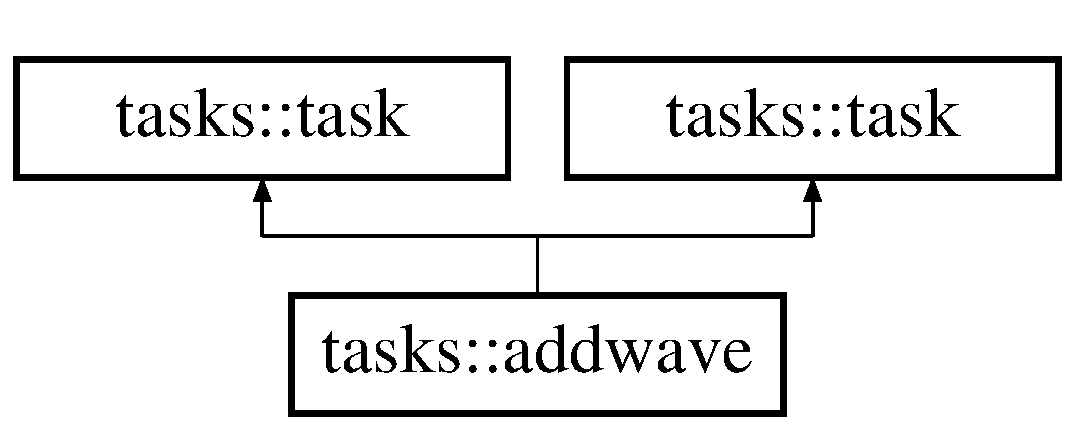
\includegraphics[height=2cm]{classtasks_1_1addwave}
\end{center}
\end{figure}
\subsection*{Public Member Functions}
\begin{CompactItemize}
\item 
def \textbf{run}\label{classtasks_1_1addwave_4a8ed1b51830f9a6271981d584b71a5e}

\item 
def \textbf{run}\label{classtasks_1_1addwave_4a8ed1b51830f9a6271981d584b71a5e}

\end{CompactItemize}
\subsection*{Static Public Attributes}
\begin{CompactItemize}
\item 
string \textbf{name} = '{\bfaddwave}'\label{classtasks_1_1addwave_50238349fcf518ca91b72579b452d0f0}

\item 
string \textbf{button\-Text} = 'Add wavelengths'\label{classtasks_1_1addwave_f035e4aefe65f969b93658538d1fd0d3}

\item 
string \textbf{suffix} = 'wave'\label{classtasks_1_1addwave_6a9791b9244d63099175839c7043fc97}

\item 
list \textbf{prereq} = ['{\bfextspec}']\label{classtasks_1_1addwave_fb86f5c9b6bff73826404872a2ecd16a}

\end{CompactItemize}


\subsection{Detailed Description}


\footnotesize\begin{verbatim}Append wavelength information to the extracted orders. The wavelength definition
   is taken from the pre-determined solution of the wavelength reference frame.
\end{verbatim}
\normalsize
 



The documentation for this class was generated from the following files:\begin{CompactItemize}
\item 
old/PANICtool-1.0/tasks.py\item 
old/tasks.py\end{CompactItemize}
